\documentclass{article}
\usepackage[utf8]{inputenc}

\title{Lecture 2: Probability }
\author{wbg231 }
\date{November 2022}
\usepackage{tikz,graphicx,amsmath,amsfonts,amscd,amssymb,bm,cite,epsfig,epsf,url}
\begin{document}

\maketitle

\section{why do we need probability}
\subsection{ language}
\begin{itemize}
    \item probability was invented to characterize uncertainty
    \item when we speak using terms like, "with high probability" or "certainly" the probability actually associated with those words can be uncertain
    \item language is to uncertain to use in science. we want something more rigorous 
\subsection{formal logic}
\item this works really well when something is always or never true, but it is hard with things that are probabilistic. 
\item if the premise is true then the conclusion should be true
\item conditional reasoning if p then q 
\item this works well for systems that are simple (or where the rules are well defined) math programming, world we create. 
\item but what about the real world?
\item what if we say "some candy is sweet" and we say "chocolate is sweet" then we can draw no conclusions 
\item there is no concept of likelihood
\item if if rained the street is wet, but if the street is wet there are other reasons why the street could be wet, but this does not characterize cases where we can say the likelyhood it rained given the street is wet is not super well defined 
\item we need something less rigid than logic and more formal than language. 
\section{Probability introduction}
\subsection{start of probability}
\item most probability started from gambling in the 1660's. mostly analyzing card and dice games
\item the emergence of probability, and the taming of chance were the first probability analysis. 
\item in the 1930's they made probability axiomatic 
\subsection{purpose of probilaity}
\item the goal is rational descion making under uncertainty 
\item we use it for inference, which is not proof. it just allows us to make choices. 
\item inference is a choice
\item but the scope can be broader. 
\itme so our running example is going to be in vitro firtilization. there is a lot of uncertanty. it is a good example for probability that people may care about 
\item pretty much all choices in invitro firtlization call this (IF)is about probability
\subsection{Case study}
\item 29 year old patient want to have patients with invitor firtizlzaiton (IVF) 
\item they produce 19 eggs.
\item all the eggs are retrieved
\item 13/19 are mature enough to attempt fertilization 
\item 11 of those are actually fertilized 
\item 8 of 11 grow fast enough to become viable 
\item at day 5 tow choices must be made, how many to biopsy and which to transfer
\item biopsy take a hang full of cells and take a sample of that to see how they might grow. 
\iem after biposy which do you implant to max your chance of having a successfully birth 
\item this is a high stake problem 
\subsection{doing this with probability}
\item this is a life and death situation 
\item but the actual computation is simple given we understand how to model the sitatuation, as well as rv and probabilitties. 
\subsection{probability defention}
\item we are going to start thinking with a combination lock 
\item the sample space is the set of all possible outcomes of a random experiment 
\item experiment- not a scientific experiment it is instead anyhting where the outcome is uncertain but it is repeatable. think about a combinaation lock you can try many difrent combinations and see the outcome 
\itme in a 1 digit combination lock our sample space is 0,9 so we have 10 outcomes
\item outcome, the result of a singe experiment 
\item event a subset of the sample space can be formed form many outcomes. ie getting all odd numbers in 3 dice rolls) 
\item proabability the relative proportion of th esample space taken up by the evne t
\item probailiy meausure a funciton mapping teh outocmes in teh sampel space from 0 to  1
\item this is super common 
\itme the naive fallacy is conducting the number of potential outcomes with the proportion of the sample space taken up by each outcome 
\item example: you apply to two colleges a safty school and a reach. You say you have a 50\% Chance of getting into either, but that is incorrect you have a higher chance of getting into 1 and a lower chance of the other-. 
\item sample space $\Omega$ all possible outocmes 
\item the event space also called the collection is the power set of all possible events. (ie every combiation of outcomes that you can get)
\item the probaility measure maps the collection or event sapce to the numbers between 0 and 1 
\item the probaility space is formed as $(\Omega, F(\text{ or }C), P)$
\item you need all three to define a probility space
\item axioms of probaility
\begin{enumerate}
    \item for every event e $P(e)\geq 0$
    \item $P(\Omega)=1$ ie the sample space defines everything that can happen (this fails in a lot of applied examples especially if things are Cauchy) 
    \item if $A,B\in C$ are disjoint then $P(A\cup B)=P(A)+P(B)$
\end{enumerate}
\item suppose that we have to events A and B if they are mtually exlusive P(A or B)=P(A)+P(B)
\item mutally exlusive meaning that they have no overalp ex are pregent or not pregent one state at a time ever.  
\item mutually exclusive does not mean that they have the same likely hood of happening 
\item the mental model that you should have is a geer. if you know something is mutally exlusive that gives you a lot of infomraiton. 
\item something about the enigma machine is all about mutually exclusive events 
\item what if the events are not muttually exlusive 
\item $A,B\in C$ are not mutually exclusive $P(A\cup B)=P(A)+P(B)-P(P\cap B)$
\item interscetion can be thought of as the joint
\item if events are independent of one another $P(A\cap B)=P(A)P(B)$
\itme otherwise ie a and b are not indpendint  $P(A\cap B)=P(A)P(B|A)$ this is directly from bayes 
\item $P(B|a)=P(A)$ in independince 
\item condtional probaility 
\item $P(B|A)-\frac{P(A|B)P(b)}{P(a)}=\frac{P(A\cap B)}{P(A)}$
\item the real point of conditional probaiblity is that the sample space changes given we know that A occoured. so how infomrative this is about the b is how A is intersected with b 
\item if A and B are not mutually exlusive or independint immage to gears that are ocnected by some thing. 
\item probabilistic thinking is not intuitive. gambeling only makes sense becase we do not get probaility
\item examples of poeple being bad at prob
\begin{enumerate}
    \item bil gates tweeted that sharks killed much less people than mosquito's every year, the issue with this is but there are many more encounters between people and mosquitoes than with sharks. so it may not be safer to be around a shark than a mosquito. this is an issue of conditional probability. it is easy to get this wrong
    \item the Monty hall problem. there are three doors, behind 1 is a prize call that door k. you pick a door call it door i, and the host shows you what is behind one of the other two doors call it door j. you you are given to switch and sellect a new door call it door l. and you want to know should you swtich. 
    \item think of it like this let w be win, switch be s, and f be first (which takes on value 1 if you pick correctly and 0 otherwise. here we can assume that switching and your first choice are indepdnint, this makes sense if that is your stat $P(w=1|s=0)=P(w=1,f=0|s=0)+P(w=1,f=1|s=0)=P(w=1|s=0,f=0)P(s=0|f=0)P(f=0)+P(w=1|s=0,f=1)P(s=0|f=1)P(f=1)=P(w=1|s=0,f=1)P(s=0|f=1)P(f=1)$ since clearly $P(w=1,f=1|s=0)=0$ if we chose wrong and did not switch  $P(w=1|s=0,f=1)P(s=0|f=1)P(f=1)=(1)(p)P(f=1)\frac{p}{3}$ where p is our liklyhood of switching 
    \item now consider $P(w=1|s=1)=P(w=1,f=0|s=1)+P(w=1,f=1|s=1)=P(w=1|f=0,s=1)P(s=1|f=0)P(f=0)+P(w=1|f=1,s=1)P(s=1|f=1)P(f=1)=P(w=1|f=0,s=1)P(s=1|f=0)P(f=0)$ since if we chose right and stich we never win $P(w=1|f=0,s=1)P(s=1|f=0)P(f=0)=(1)(p)\frac{2}{3}$
    \item $P(w=1|s=1)=\frac{2p}{3}$ and $P(w=1|s=0)=\frac{p}{3}$
    \item we can maximise this by setting p=1 that is by always switching in this case we have a 2/3 cahnce of wining. 
\end{enumerate}
\item gardener example 
\begin{itemize}
    \item someone has two children and you know the older one is a girl 
    \item what is the liklyhood all children are girls 
    \item we assume that the liklyhood of being either gender is euqla 
    \itme and we also assume independince between the gender of each child. 
    \item so we want $P(g_1=1,g_2=1|g_1=1)\frac{P(g_1=1,g_2=1,g_2=2)}{P(g_2=1)}=\frac{P(g_1=1,g_2=2}{P(g_2=1)}=\frac{\frac{1}{2}\frac{1}{2}}{\frac{1}{2}}=\frac{1}{2}$
    \item what if we know that at least one of the children is a girl. $P(g_1=1,g_2=1)|(g_1=1\cup g_2=1)=\frac{(g_1=1,g_2=1)\cap(g_1=1\cup g_2=1)}{P(g_1=1\cup g_2=1)}=\frac{P(g_1=1,g_2=2)}{P(g_1=1 \cup g_2=1)}=\frac{\frac{1}{4}}{\frac{3}{4}}=\frac{1}{3}$
\end{itemize}
\subsection{Probability distributions }
\item there is a company that says, "they guarantee you will have a child". how can they give such a guarantee? 
\item uniform distribution: $\forall x \in \Omega P(x)=\frac{1}{|\Omega|}$ ie all outcomes equally likely 
\item 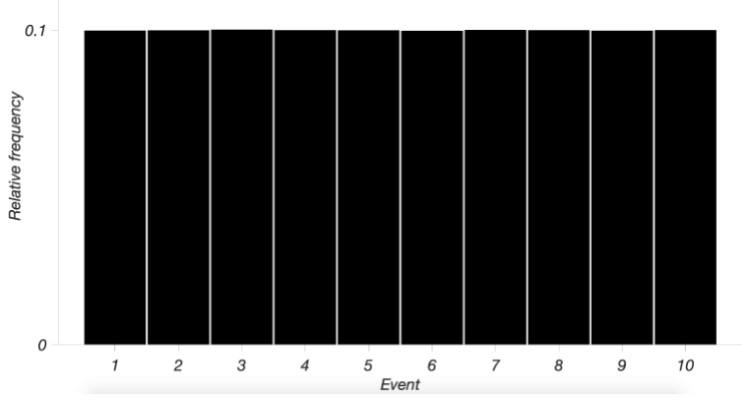
\includegraphics[width=15cm]{Final_Review/Lecture_2/uniform_1.jpg}

\item question: immagine an rv x that is unfirom between 1 and 10, and two rvs y,z that are unfirom between 1 and 5

\item are the distribution of x and y+z=a the same? no the sample space has changed 
\item x and y can each take values between 1 and 5, so there are 25 unique combinations. where are x only has 10
\item so consider P(x=10)=\frac{1}{10}
\item P(a=10)=P(x=5,y=5)=P(x=5|y=5)P(y=5)=\frac{1}{5}\frac{1}{5}=\frac{1}{25}
\item so the sum of two uniform y and z look like this 
\item 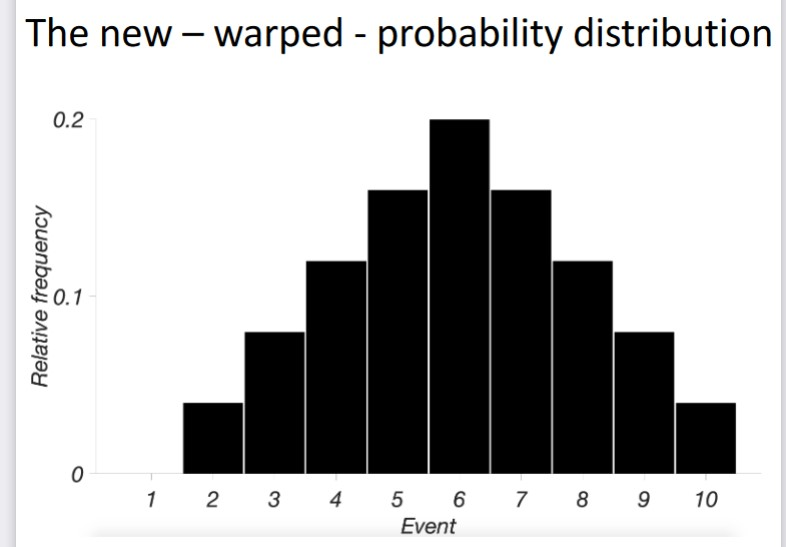
\includegraphics[width=15cm]{Final_Review/Lecture_2/two_uniform.jpg}
\item so the extremes are less likely 
\item this is a warrped probability distorbution 
\item so we can make concluisons that are almost triviall bassed on this. 
\item then he talks about dream for a while
\item running somethign that is unfiform many times, getting extreme outcomes becomes very unlikely very quickly 
\item the house does not always win, it just always wins in the long run 
\item insurance contracts only really works with uncorelated evetns
\subsection{random variables}
\item x+3=10, in this case x is a constant the only values that holds is x=7
\item y=x+5 x is a vairble ie it can take any value
\item given this what is a random vairble 
\item a random varible is 
\item A radnom vairble a is a function $a:\Omega\rightarrow \mathbb{R}$ ie it maps from the sample space to the real number. 
\item but functions are deterministic where does the randomness come from? 
\item it comes from the sample space, which is the outcome of a random experiment  
\item a random vairble is neither random nor a vairble 
\subsection{ back to exmaple}
\item 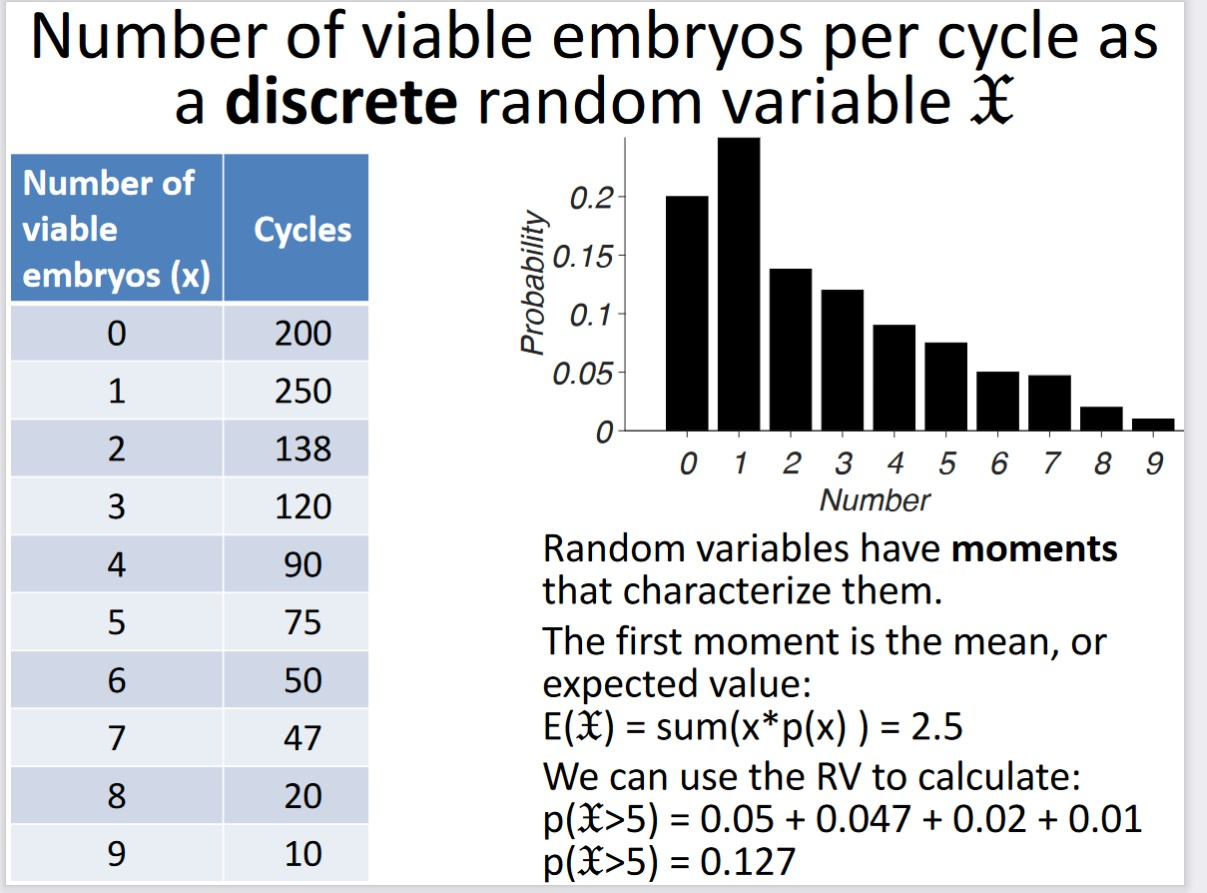
\includegraphics[width=15cm]{Final_Review/Lecture_2/lecture_1example.jpg}


\item we are working for an IVF firm. we run a cycle and record the numebr fo viable embroys
\item the outocme of any given cycle is uncertian 
\item but we can charciterize the process 
\item our sample space is $\mathbb{Z}$ that is in princple we could have any integer number of viable emberyos
\item we are not going to make assumptions about this we are looking at the data, there are empyrically 1000 samples recorded. 
\item row coresponds to outcome 
\item cycclesa are the  number of cycles that took on that vlaue 
\itme P(x=x) is the fraction of times occoured/ 
\item so we can see there is the probaility mass function 
\itme a random vairble has a pmf but is nto equla to its pmf
\itme so we charictrize a rv with its pmf and moments 
\item the first moment of a rv is its expected value
\item so we can use this distrobution to charicterize how we can make a garuntee, we can say proabbilitsticllt this will happen. 

\end{itemize}

\end{document}
